% ============================================================
%  template.tex —— 主文件，只写内容
%  编译方式：XeLaTeX（支持中文），编译两次生成目录
% ============================================================
\documentclass[notheorems]{beamer}

\input{pptheader.tex}
\input{mycommand.tex}

\begin{document}
	
	% ============================================================
	%  元信息：修改标题、作者、单位、日期
	% ============================================================
	\title[科研汇报]{基于高阶有限元的变密度拓扑优化}
	\subtitle{博士期间科研工作汇报}
	
	% 在 [] 中填入短作者名，避免把导师信息和排版命令也带入页脚
	\author[何亮]{报告人：何亮 \\
		\vspace{5pt}
		导师：{\CJKfontspec{SimSun}魏华祎} 教授}
	
	% [] 中填入单位简称
	\institute[湘大数学院]{
		\vspace{5pt}
		湘潭大学 \\
		数学与计算科学学院
	}
	\date{\today}
	
	% ---- 封面页 ----
	\frame[plain]{\titlepage}
	
	% ============================================================
	%  个人简介页（封面与目录之间）
	% ============================================================
	\begin{frame}[plain]
		
		\begin{tikzpicture}[remember picture, overlay]
			\fill[structure.fg]
			(current page.north west)
			rectangle ([yshift=-0.077\paperheight] current page.north east);
			\node[white, anchor=west, font=\small\bfseries\sffamily]
			at ([xshift=0.025\paperwidth, yshift=-0.038\paperheight]
			current page.north west)
			{个人简介};
			\fill[panelbg]
			([yshift=-0.077\paperheight] current page.north west)
			rectangle ([xshift=0.38\paperwidth] current page.south west);
		\end{tikzpicture}
		
		\vspace{0.077\paperheight}
		
		\begin{columns}[T, totalwidth=\linewidth]
			
			% ══════════════════════════════════════════
			% 左栏：照片 + 姓名 + 研究方向
			% ══════════════════════════════════════════
			\begin{column}{0.36\linewidth}
				\vspace{0.5em}
				\begin{center}
					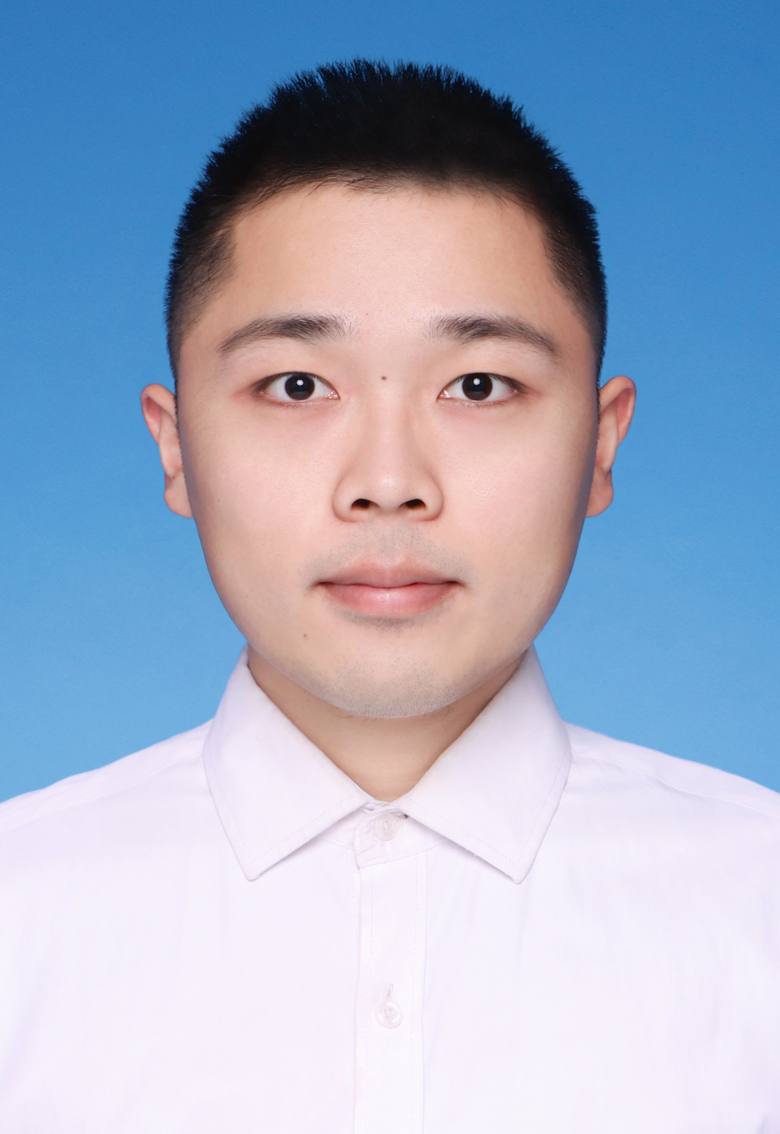
\includegraphics[width=0.50\linewidth,
					height=0.22\paperheight,
					keepaspectratio]{photo.jpg}
					
					\vspace{0.3em}
					{\fontsize{14}{18}\selectfont\bfseries\sffamily 何\quad 亮}
					
					\vspace{0.5em}
					\begin{tcolorbox}[
						colback=structure.fg, colframe=structure.fg,
						arc=4pt, boxrule=0pt,
						top=3pt, bottom=3pt, left=6pt, right=6pt,
						width=0.78\linewidth]
						\centering\color{white}\bfseries\small\sffamily 研究方向
					\end{tcolorbox}
					
					\vspace{4pt}
					% 标签：缩小字号与内边距，紧凑排列
					\tcbox[on line, arc=4pt, colback=white, colframe=tagborder,
					boxrule=0.8pt, top=1.5pt, bottom=1.5pt, left=5pt, right=5pt,
					fontupper=\footnotesize\bfseries\sffamily\color{structure.fg}]
					{偏微分方程数值方法}\\[3pt]
					\tcbox[on line, arc=4pt, colback=white, colframe=tagborder,
					boxrule=0.8pt, top=1.5pt, bottom=1.5pt, left=5pt, right=5pt,
					fontupper=\footnotesize\bfseries\sffamily\color{structure.fg}]
					{连续体结构拓扑优化}\\[3pt]
					\tcbox[on line, arc=4pt, colback=white, colframe=tagborder,
					boxrule=0.8pt, top=1.5pt, bottom=1.5pt, left=5pt, right=5pt,
					fontupper=\footnotesize\bfseries\sffamily\color{structure.fg}]
					{科学计算软件设计与实现}
				\end{center}
			\end{column}
			
			% ══════════════════════════════════════════
			% 右栏：研究主线 + 研究目标
			% ══════════════════════════════════════════
			\begin{column}{0.62\linewidth}
				\vspace{0.5em}
				
				% ── 研究主线 ────────────────────────────
				\begin{tcolorbox}[
					colback=structure.fg, colframe=structure.fg,
					arc=4pt, boxrule=0pt,
					top=3pt, bottom=3pt, left=8pt, right=8pt,
					width=\linewidth]
					\centering\color{white}\bfseries\small\sffamily 研究主线
				\end{tcolorbox}
				
				\vspace{3pt}
				{\fontsize{7.5}{10}\selectfont
					围绕基于高阶有限元的变密度拓扑优化开展系统研究，重点关注四个方面：}
				
				\vspace{4pt}
				% ── 2×2 网格 ────────────────────────────
				% 用 tabular + minipage 解决宽度与换行问题
				\begin{tabular}{@{}l@{\hspace{4pt}}l@{}}
					% 第一行
					\circnum{01}~%
					\begin{minipage}[c]{2.6cm}
						\begin{tcolorbox}[colback=panelbg!50, colframe=panelbg,
							arc=2pt, boxrule=0.5pt,
							top=2pt, bottom=2pt, left=4pt, right=4pt, nobeforeafter]
							\fontsize{7}{9}\selectfont 高阶有限元拓扑优化方法
						\end{tcolorbox}
					\end{minipage}
					&
					\circnum{03}~%
					\begin{minipage}[c]{2.6cm}
						\begin{tcolorbox}[colback=panelbg!50, colframe=panelbg,
							arc=2pt, boxrule=0.5pt,
							top=2pt, bottom=2pt, left=4pt, right=4pt, nobeforeafter]
							\fontsize{7}{9}\selectfont 胡张混合有限元拓扑优化方法
						\end{tcolorbox}
					\end{minipage}
					\\[6pt]
					% 第二行
					\circnum{02}~%
					\begin{minipage}[c]{2.6cm}
						\begin{tcolorbox}[colback=panelbg!50, colframe=panelbg,
							arc=2pt, boxrule=0.5pt,
							top=2pt, bottom=2pt, left=4pt, right=4pt, nobeforeafter]
							\fontsize{7}{9}\selectfont 多分辨率拓扑优化框架
						\end{tcolorbox}
					\end{minipage}
					&
					\circnum{04}~%
					\begin{minipage}[c]{2.6cm}
						\begin{tcolorbox}[colback=panelbg!50, colframe=panelbg,
							arc=2pt, boxrule=0.5pt,
							top=2pt, bottom=2pt, left=4pt, right=4pt, nobeforeafter]
							\fontsize{7}{9}\selectfont SOPTX 软件平台设计与实现
						\end{tcolorbox}
					\end{minipage}
				\end{tabular}
				
				\vspace{6pt}
				% ── 研究目标 ────────────────────────────
				\begin{tcolorbox}[
					colback=structure.fg, colframe=structure.fg,
					arc=4pt, boxrule=0pt,
					top=3pt, bottom=3pt, left=8pt, right=8pt,
					width=\linewidth]
					\centering\color{white}\bfseries\small\sffamily 研究目标
				\end{tcolorbox}
				
				\vspace{4pt}
				{\fontsize{8}{11}\selectfont
					面向复杂结构轻量化设计需求，围绕高精度分析、高效优化求解与软件平台实现，提升连续体结构拓扑优化的理论研究水平与工程应用能力。}
				
			\end{column}
		\end{columns}
	\end{frame}
	
	% ---- 每节开始自动插入目录页 ----
	\AtBeginSection[]{
		\frame<beamer>{
			\frametitle{目录}
			\tableofcontents[currentsection]
		}
	}
	
	% ---- 全局目录（可选） ----
	\begin{frame}
		\frametitle{目录}
		\tableofcontents
	\end{frame}
	
	
	% ============================================================
	\section{研究背景与关键问题}
	% ============================================================
	
	% ============================================================
	%  01-1  研究背景
	% ============================================================
	\begin{frame}
		\frametitle{研究背景}
		
		% ══════════════════════════════════════════════════════════
		%  中部图片区：三图横向并列，统一外框尺寸 + 居中对齐
		% ══════════════════════════════════════════════════════════
		\begin{columns}[T, totalwidth=\linewidth]
			
			\begin{column}{0.32\linewidth}
				\begin{tcolorbox}[
					enhanced, nobeforeafter,
					colback=white, colframe=structure.fg!25,
					boxrule=0.4pt, arc=2pt,
					left=3pt, right=3pt, top=4pt, bottom=4pt,
					width=\linewidth, height=0.40\paperheight,
					halign=center,
					]
					\centering
					\begin{minipage}[c][0.27\paperheight][c]{\linewidth}
						\centering
						
\includegraphics[width=\linewidth,
						height=0.27\paperheight, keepaspectratio]{aerospace}
					\end{minipage}
					\par\vspace{8pt}
					{\footnotesize\sffamily 航空航天承力结构}
				\end{tcolorbox}
			\end{column}
			
			\begin{column}{0.32\linewidth}
				\begin{tcolorbox}[
					enhanced, nobeforeafter,
					colback=white, colframe=structure.fg!25,
					boxrule=0.4pt, arc=2pt,
					left=3pt, right=3pt, top=4pt, bottom=4pt,
					width=\linewidth, height=0.40\paperheight,
					halign=center,
					]
					\centering
					\begin{minipage}[c][0.27\paperheight][c]{\linewidth}
						\centering
						
\includegraphics[width=\linewidth,
						height=0.27\paperheight, keepaspectratio]{building}
					\end{minipage}
					\par\vspace{8pt}
					{\footnotesize\sffamily 高层建筑抗侧力体系}
				\end{tcolorbox}
			\end{column}
			
			\begin{column}{0.32\linewidth}
				\begin{tcolorbox}[
					enhanced, nobeforeafter,
					colback=white, colframe=structure.fg!25,
					boxrule=0.4pt, arc=2pt,
					left=3pt, right=3pt, top=4pt, bottom=4pt,
					width=\linewidth, height=0.40\paperheight,
					halign=center,
					]
					\centering
					\begin{minipage}[c][0.27\paperheight][c]{\linewidth}
						\centering
						
\includegraphics[width=\linewidth,
						height=0.27\paperheight, keepaspectratio]{biomedical}
					\end{minipage}
					\par\vspace{8pt}
					{\footnotesize\sffamily 个性化生物医疗植入体}
				\end{tcolorbox}
			\end{column}
			
		\end{columns}
		
		\vspace{1em}
		
		% ══════════════════════════════════════════════════════════
		%  底部文字区：三条递进式结论，1/2/3 编号，左对齐
		%  采用 \makebox + \parbox 组合保证编号列与正文列精准对齐
		% ══════════════════════════════════════════════════════════
		{\fontsize{8.5}{14}\selectfont\sffamily
			\noindent
			\makebox[1.5em][l]{\textbf{1}}%
			\parbox[t]{\dimexpr\linewidth - 1.5em\relax}{%
				复杂工程结构设计对轻量化、高性能与高可靠性提出了更高要求}
			
			\vspace{5pt}\noindent
			\makebox[1.5em][l]{\textbf{2}}%
			\parbox[t]{\dimexpr\linewidth - 1.5em\relax}{%
				结构优化设计经历了由尺寸优化、形状优化到拓扑优化的递进发展}
			
			\vspace{5pt}\noindent
			\makebox[1.5em][l]{\textbf{3}}%
			\parbox[t]{\dimexpr\linewidth - 1.5em\relax}{%
				连续体结构拓扑优化以设计域内材料分布作为核心设计变量，
				是复杂结构性能驱动设计的重要数学工具}
		}
		
	\end{frame}
	
	% ============================================================
	%  01-2  关键问题
	% ============================================================
	\begin{frame}
		\frametitle{关键问题}
		
		% ── 总述条 ───────────────────────────────────────────────
		\begin{tcolorbox}[
			colback=panelbg, colframe=structure.fg!40,
			arc=3pt, boxrule=0.5pt,
			top=3pt, bottom=3pt, left=8pt, right=8pt]
			{\fontsize{8}{12}\selectfont\sffamily
				面向复杂工程应用，连续体结构拓扑优化仍面临
				高精度分析、高分辨率设计、复杂局部约束与统一软件实现等关键挑战。}
		\end{tcolorbox}
		
		\vspace{-1.2em}  % 顶部总述条与卡片之间的负间距
		
		% ── 第一行 ───────────────────────────────────────────────
		\begin{columns}[T, totalwidth=\linewidth]
			
			\begin{column}{0.485\linewidth}
				\begin{tcolorbox}[
					colback=white, colframe=structure.fg!50,
					colbacktitle=structure.fg, coltitle=white,
					fonttitle=\fontsize{8}{10}\selectfont\bfseries\sffamily,
					title={\circnum{01}\enspace 局部力学场刻画精度受限},
					arc=3pt, boxrule=0.5pt,
					toptitle=0.25pt, bottomtitle=0.25pt,
					top=3pt, bottom=3pt, left=6pt, right=6pt]
					{\fontsize{7.5}{11}\selectfont\sffamily
						\begin{itemize}
							\setlength{\itemsep}{1pt}
							\setlength{\topsep}{1pt}
							\setlength{\parsep}{0pt}
							\setlength{\parskip}{0pt}
							\item 传统低阶位移元对复杂变形与局部应力场的刻画能力有限
							\item 应力场精度不足，影响灵敏度分析与约束评估可靠性
					\end{itemize}}
				\end{tcolorbox}
			\end{column}
			
			\begin{column}{0.485\linewidth}
				\begin{tcolorbox}[
					colback=white, colframe=structure.fg!50,
					colbacktitle=structure.fg, coltitle=white,
					fonttitle=\fontsize{8}{10}\selectfont\bfseries\sffamily,
					title={\circnum{02}\enspace 分辨率与规模难以兼顾},
					arc=3pt, boxrule=0.5pt,
					toptitle=0.25pt, bottomtitle=0.25pt,
					top=3pt, bottom=3pt, left=6pt, right=6pt]
					{\fontsize{7.5}{11}\selectfont\sffamily
					\begin{itemize}
							\setlength{\itemsep}{1pt}
							\setlength{\topsep}{1pt}
							\setlength{\parsep}{0pt}
							\setlength{\parskip}{0pt}
							\item 高分辨率设计有助于获得边界清晰、细节丰富的构型
							\item 单分辨率框架下，分辨率提高通常伴随计算规模增长
					\end{itemize}}
				\end{tcolorbox}
			\end{column}
			
		\end{columns}
		
		% ── 第二行 ───────────────────────────────────────────────
		\begin{columns}[T, totalwidth=\linewidth]
			
			\begin{column}{0.485\linewidth}
				\begin{tcolorbox}[
					colback=white, colframe=structure.fg!50,
					colbacktitle=structure.fg, coltitle=white,
					fonttitle=\fontsize{8}{10}\selectfont\bfseries\sffamily,
					title={\circnum{03}\enspace 局部应力约束建模与求解困难},
					arc=3pt, boxrule=0.5pt,
					toptitle=0.25pt, bottomtitle=0.25pt,
					top=3pt, bottom=3pt, left=6pt, right=6pt]
					{\fontsize{7.5}{11}\selectfont\sffamily
					\begin{itemize}
							\setlength{\itemsep}{1pt}
							\setlength{\topsep}{1pt}
							\setlength{\parsep}{0pt}
							\setlength{\parskip}{0pt}
							\item 局部应力约束存在应力奇异性，建模与灵敏度分析困难
							\item 大量局部约束易导致优化求解困难与迭代不稳定
					\end{itemize}}
				\end{tcolorbox}
			\end{column}
			
			\begin{column}{0.485\linewidth}
				\begin{tcolorbox}[
					colback=white, colframe=structure.fg!50,
					colbacktitle=structure.fg, coltitle=white,
					fonttitle=\fontsize{8}{10}\selectfont\bfseries\sffamily,
					title={\circnum{04}\enspace 缺乏统一软件实现框架},
					arc=3pt, boxrule=0.5pt,
					toptitle=0.25pt, bottomtitle=0.25pt,
					top=3pt, bottom=3pt, left=6pt, right=6pt]
					{\fontsize{7.5}{11}\selectfont\sffamily
					\begin{itemize}
							\setlength{\itemsep}{1pt}
							\setlength{\topsep}{1pt}
							\setlength{\parsep}{0pt}
							\setlength{\parskip}{0pt}
							\item 先进数值方法与高性能计算机制缺乏统一实现框架
							\item 自动微分、多后端切换与 CPU/GPU 异构支持仍显不足
					\end{itemize}}
				\end{tcolorbox}
			\end{column}
			
		\end{columns}
		
	\end{frame}
	
	
	% ============================================================
	\section{高精度拓扑优化数值方法}
	% ============================================================
	
	% ============================================================
	%  02-1  从高阶离散到混合建模
	% ============================================================
	\begin{frame}
		\frametitle{从高阶离散到混合建模}
		
		% ── 顶部总述条 ───────────────────────────────────────────
		\begin{tcolorbox}[
			colback=panelbg, colframe=structure.fg!40,
			arc=3pt, boxrule=0.5pt,
			top=3pt, bottom=3pt, left=8pt, right=8pt]
			{\fontsize{8}{12}\selectfont\sffamily
				围绕“精度—效率—约束”三个核心问题，构建系统性高精度拓扑优化数值方法。}
		\end{tcolorbox}
		
		\vspace{-1.2em}
		
		% ══════════════════════════════════════════════════════════
		%  主体双栏：左侧关键问题 / 右侧方法路径
		% ══════════════════════════════════════════════════════════
		\begin{columns}[T, totalwidth=\linewidth]
			
			% ─── 左栏：关键科学问题 ───────────────────────────
			\begin{column}{0.485\linewidth}
				\begin{tcolorbox}[
					colback=white, colframe=structure.fg!50,
					colbacktitle=structure.fg, coltitle=white,
					fonttitle=\fontsize{8}{10}\selectfont\bfseries\sffamily,
					title={关键科学问题},
					arc=3pt, boxrule=0.5pt,
					toptitle=3pt, bottomtitle=3pt,
					top=5pt, bottom=5pt, left=6pt, right=6pt]
					{\fontsize{7.5}{11}\selectfont\sffamily
						\setbeamertemplate{enumerate item}{\fontsize{5.5}{7}\selectfont\circnum{0\insertenumlabel}}
						\begin{enumerate}
							\setlength{\itemsep}{6pt}
							\setlength{\topsep}{0pt}
							\setlength{\parsep}{0pt}
							\setlength{\parskip}{0pt}
							
							\item 局部力学场刻画精度受限，传统低阶位移元对局部应力场刻画能力有限
							
							\item 设计分辨率与规模难以兼顾，细网格带来巨大计算与存储开销
							
							\item 局部应力约束建模与求解困难，应力奇异性、局部性与大量约束并存
						\end{enumerate}
					}
				\end{tcolorbox}
			\end{column}
			
			% ─── 右栏：方法路径与技术贡献 ─────────────────────
			\begin{column}{0.485\linewidth}
				\begin{tcolorbox}[
					colback=white, colframe=structure.fg!50,
					colbacktitle=structure.fg, coltitle=white,
					fonttitle=\fontsize{8}{10}\selectfont\bfseries\sffamily,
					title={方法路径与技术贡献},
					arc=3pt, boxrule=0.5pt,
					toptitle=3pt, bottomtitle=3pt,
					top=5pt, bottom=5pt, left=6pt, right=6pt]
					{\fontsize{7.5}{11}\selectfont\sffamily
						\setbeamertemplate{enumerate item}{\fontsize{5.5}{7}\selectfont\circnum{0\insertenumlabel}}
						\begin{enumerate}
							\setlength{\itemsep}{6pt}
							\setlength{\topsep}{0pt}
							\setlength{\parsep}{0pt}
							\setlength{\parskip}{0pt}
							
							\item 任意次拉格朗日有限元方法，提升位移场及其派生应力场逼近精度
							
							\item 高阶有限元多分辨率拓扑优化框架，解耦分析网格与设计变量
							
							\item 任意次胡张混合有限元方法，直接逼近应力场，支撑局部约束可靠评估
						\end{enumerate}
					}
				\end{tcolorbox}
			\end{column}
			
		\end{columns}
		
		\vspace{0.5em}
		
		% ── 底部结论条 ───────────────────────────────────────────
		\begin{tcolorbox}[
			colback=structure.fg, colframe=structure.fg,
			arc=3pt, boxrule=0pt,
			top=4pt, bottom=4pt, left=8pt, right=8pt]
			\centering
			{\fontsize{8.5}{12}\selectfont\sffamily\color{white}
				形成\textbf{“高阶离散 — 多分辨率解耦 — 混合应力建模}"的高精度拓扑优化方法体系}
		\end{tcolorbox}
		
	\end{frame}
	
	% ============================================================
	%  02-2  任意次拉格朗日有限元拓扑优化方法
	% ============================================================
	\begin{frame}
		\frametitle{任意次拉格朗日有限元拓扑优化方法}
		
		% ── 顶部总述条 ───────────────────────────────────────────
		\begin{tcolorbox}[
			colback=panelbg, colframe=structure.fg!40,
			arc=3pt, boxrule=0.5pt,
			top=3pt, bottom=3pt, left=8pt, right=8pt]
			{\fontsize{8}{12}\selectfont\sffamily
				将变密度拓扑优化中的状态方程从传统低阶位移元推广到任意次拉格朗日有限元，
				构建统一的高阶离散与优化建模框架。}
		\end{tcolorbox}
		
		\vspace{-1.0em}
		
		% ── 三列卡片 ─────────────────────────────────────────────
		\begin{columns}[T, totalwidth=\linewidth]
			
			% ─── 01 高阶有限元离散 ────────────────────────────
			\begin{column}{0.325\linewidth}
				\begin{tcolorbox}[
					colback=white, colframe=structure.fg!50,
					colbacktitle=structure.fg, coltitle=white,
					fonttitle=\fontsize{8}{10}\selectfont\bfseries\sffamily,
					title={\circnum{01}\enspace 任意次有限元离散},
					arc=3pt, boxrule=0.5pt,
					toptitle=0.25pt, bottomtitle=0.25pt,
					top=3pt, bottom=3pt, left=6pt, right=6pt]
					{\fontsize{7.5}{11}\selectfont\sffamily
					\setbeamertemplate{itemize item}{\raisebox{1pt}{\tiny$\bullet$}}
					\setlength{\leftmargini}{0.85em}
						\begin{itemize}
							\setlength{\itemsep}{2pt}
							\setlength{\topsep}{1pt}
							\setlength{\parsep}{0pt}
							\setlength{\parskip}{0pt}
							\item 基于线弹性弱形式建立密度参数化状态方程
							\item 构造任意次拉格朗日有限元空间 $V_h^k$
							\item 统一支持单纯形单元与张量积单元
					\end{itemize}}
				\end{tcolorbox}
			\end{column}
			
			% ─── 02 设计变量表征 ──────────────────────────────
			\begin{column}{0.325\linewidth}
				\begin{tcolorbox}[
					colback=white, colframe=structure.fg!50,
					colbacktitle=structure.fg, coltitle=white,
					fonttitle=\fontsize{8}{10}\selectfont\bfseries\sffamily,
					title={\circnum{02}\enspace 设计变量表征},
					arc=3pt, boxrule=0.5pt,
					toptitle=0.25pt, bottomtitle=0.25pt,
					top=3pt, bottom=3pt, left=6pt, right=6pt]
					{\fontsize{7.5}{11}\selectfont\sffamily
					\setbeamertemplate{itemize item}{\raisebox{1pt}{\tiny$\bullet$}}
					\setlength{\leftmargini}{0.85em}
						\begin{itemize}
							\setlength{\itemsep}{2pt}
							\setlength{\topsep}{1pt}
							\setlength{\parsep}{0pt}
							\setlength{\parskip}{0pt}
							\item 单元密度表征：每个单元对应一个设计变量
							\item 节点密度表征：由节点变量插值构造连续密度场
							\item SIMP 材料插值：建立密度—刚度耦合关系
					\end{itemize}}
				\end{tcolorbox}
			\end{column}
			
			% ─── 03 统一比较框架 ──────────────────────────────
			\begin{column}{0.325\linewidth}
				\begin{tcolorbox}[
					colback=white, colframe=structure.fg!50,
					colbacktitle=structure.fg, coltitle=white,
					fonttitle=\fontsize{8}{10}\selectfont\bfseries\sffamily,
					title={\circnum{03}\enspace 统一比较框架},
					arc=3pt, boxrule=0.5pt,
					toptitle=0.25pt, bottomtitle=0.25pt,
					top=3pt, bottom=3pt, left=6pt, right=6pt]
					{\fontsize{7.5}{11}\selectfont\sffamily
					\setbeamertemplate{itemize item}{\raisebox{1pt}{\tiny$\bullet$}}
					\setlength{\leftmargini}{0.85em}
						\begin{itemize}
							\setlength{\itemsep}{2pt}
							\setlength{\topsep}{1pt}
							\setlength{\parsep}{0pt}
							\setlength{\parskip}{0pt}
							\item 统一载荷、边界条件、体积约束与过滤半径
							\item 比较单元类型、离散阶次与密度表征方式
							\item 评估优化构型、收敛行为与计算代价
					\end{itemize}}
				\end{tcolorbox}
			\end{column}
			
		\end{columns}
		
		\vspace{0.5em}
		
		% ── 底部总结条 ───────────────────────────────────────────
		\begin{tcolorbox}[
			colback=structure.fg, colframe=structure.fg,
			arc=3pt, boxrule=0pt,
			top=4pt, bottom=4pt, left=8pt, right=8pt]
			\centering
			{\fontsize{8.5}{12}\selectfont\sffamily\color{white}
				为系统评估高阶有限元在变密度拓扑优化中的适用性与局限性提供统一计算框架}
		\end{tcolorbox}
		
	\end{frame}
	
	% ============================================================
	%  02-3  不同离散阶次与密度表征的比较
	% ============================================================
	\begin{frame}
		\frametitle{不同离散阶次与密度表征的比较}
		
		% ── 顶部总述条：文字随 overlay 切换 ─────────────────────
		\begin{tcolorbox}[
			colback=panelbg, colframe=structure.fg!40,
			arc=3pt, boxrule=0.5pt,
			top=3pt, bottom=3pt, left=8pt, right=8pt]
			{\fontsize{8}{12}\selectfont\sffamily
				\only<1>{在统一过滤半径与体积约束下，比较线性元（$k=1$）
					与四阶元（$k=4$）对优化构型及物理场精度的影响。}%
				\only<2>{在相同离散阶次与过滤半径下，比较单元密度表征与节点密度表征
					对边界平滑性、收敛行为与离散稳定性的影响。}%
				\only<3>{系统比较表明：高阶离散、密度表征与显式正则化三者共同决定
					优化质量，单一要素的提升不足以克服设计分辨率瓶颈。}}
		\end{tcolorbox}
		
		\vspace{-1.5em}
		
		% ── 主体内容区：overlayarea 锁高，防止版面跳动 ───────────
		\begin{overlayarea}{\linewidth}{0.50\paperheight}
			
			% ── Overlay 1：离散阶次比较 k=1 vs k=4 ───────────────────
			\only<1>{%
				\begin{columns}[T, totalwidth=\linewidth]
					
					\begin{column}{0.485\linewidth}
						\begin{tcolorbox}[
							colback=white, colframe=structure.fg!50,
							colbacktitle=structure.fg, coltitle=white,
							fonttitle=\fontsize{8}{10}\selectfont\bfseries\sffamily,
							title={线性元 \quad $k = 1$},
							arc=3pt, boxrule=0.5pt,
							toptitle=0.25pt, bottomtitle=0.25pt,
							top=5pt, bottom=5pt, left=6pt, right=6pt]
							\begin{center}
								
\includegraphics[width=0.85\linewidth,
								height=0.26\paperheight, keepaspectratio]{topo_k1}
							\end{center}
							\vspace{2pt}
							{\fontsize{7.5}{11}\selectfont\sffamily
								\setbeamertemplate{itemize item}{\raisebox{1pt}{\tiny$\bullet$}}
								\setlength{\leftmargini}{0.85em}
								\begin{itemize}
									\setlength{\itemsep}{2pt}\setlength{\topsep}{1pt}
									\setlength{\parsep}{0pt}\setlength{\parskip}{0pt}
									\item 构型轮廓模糊，边界呈锯齿状
									\item 局部应力场逼近误差较大
									\item 灵敏度分布受低精度位移场影响
							\end{itemize}}
						\end{tcolorbox}
					\end{column}
					
					\begin{column}{0.485\linewidth}
						\begin{tcolorbox}[
							colback=white, colframe=structure.fg!50,
							colbacktitle=structure.fg, coltitle=white,
							fonttitle=\fontsize{8}{10}\selectfont\bfseries\sffamily,
							title={四阶元 \quad $k = 4$},
							arc=3pt, boxrule=0.5pt,
							toptitle=0.25pt, bottomtitle=0.25pt,
							top=5pt, bottom=5pt, left=6pt, right=6pt]
							\begin{center}
								
\includegraphics[width=0.85\linewidth,
								height=0.26\paperheight, keepaspectratio]{topo_k4}
							\end{center}
							\vspace{2pt}
							{\fontsize{7.5}{11}\selectfont\sffamily
								\setbeamertemplate{itemize item}{\raisebox{1pt}{\tiny$\bullet$}}
								\setlength{\leftmargini}{0.85em}
								\begin{itemize}
									\setlength{\itemsep}{2pt}\setlength{\topsep}{1pt}
									\setlength{\parsep}{0pt}\setlength{\parskip}{0pt}
									\item 相同网格下物理场逼近精度显著提升
									\item 灵敏度分布更光滑，迭代收敛更稳定
									\item 构型与 $k=1$ 高度相似，设计分辨率未见改善
							\end{itemize}}
						\end{tcolorbox}
					\end{column}
					
				\end{columns}
			}% end only<1>
			
			% ── Overlay 2：密度表征比较 ───────────────────────────────
			\only<2>{%
				\begin{columns}[T, totalwidth=\linewidth]
					
					\begin{column}{0.485\linewidth}
						\begin{tcolorbox}[
							colback=white, colframe=structure.fg!50,
							colbacktitle=structure.fg, coltitle=white,
							fonttitle=\fontsize{8}{10}\selectfont\bfseries\sffamily,
							title={\circnum{01}\enspace 单元密度表征},
							arc=3pt, boxrule=0.5pt,
							toptitle=0.25pt, bottomtitle=0.25pt,
							top=5pt, bottom=5pt, left=6pt, right=6pt]
							\begin{center}
								
\includegraphics[width=0.85\linewidth,
								height=0.26\paperheight, keepaspectratio]{topo_elem_density}
							\end{center}
							\vspace{2pt}
							{\fontsize{7.5}{11}\selectfont\sffamily
								\setbeamertemplate{itemize item}{\raisebox{1pt}{\tiny$\bullet$}}
								\setlength{\leftmargini}{0.85em}
								\begin{itemize}
									\setlength{\itemsep}{2pt}\setlength{\topsep}{1pt}
									\setlength{\parsep}{0pt}\setlength{\parskip}{0pt}
									\item 每单元一个设计变量，实现简单
									\item 密度场分片常数，边界呈阶梯状
									\item 高阶元下插值与密度分辨率不匹配
							\end{itemize}}
						\end{tcolorbox}
					\end{column}
					
					\begin{column}{0.485\linewidth}
						\begin{tcolorbox}[
							colback=white, colframe=structure.fg!50,
							colbacktitle=structure.fg, coltitle=white,
							fonttitle=\fontsize{8}{10}\selectfont\bfseries\sffamily,
							title={\circnum{02}\enspace 节点密度表征},
							arc=3pt, boxrule=0.5pt,
							toptitle=0.25pt, bottomtitle=0.25pt,
							top=5pt, bottom=5pt, left=6pt, right=6pt]
							\begin{center}
								
\includegraphics[width=0.85\linewidth,
								height=0.26\paperheight, keepaspectratio]{topo_node_density}
							\end{center}
							\vspace{2pt}
							{\fontsize{7.5}{11}\selectfont\sffamily
								\setbeamertemplate{itemize item}{\raisebox{1pt}{\tiny$\bullet$}}
								\setlength{\leftmargini}{0.85em}
								\begin{itemize}
									\setlength{\itemsep}{2pt}\setlength{\topsep}{1pt}
									\setlength{\parsep}{0pt}\setlength{\parskip}{0pt}
									\item 节点插值构造连续密度场，边界更光滑
									\item 与高阶元空间自然相容，稳定性更好
									\item 灵敏度分析需额外处理插值雅可比项
							\end{itemize}}
						\end{tcolorbox}
					\end{column}
					
				\end{columns}
			}% end only<2>
			
			% ── Overlay 3：综合结论三列卡片 ──────────────────────────
			\only<3>{%
				\begin{columns}[T, totalwidth=\linewidth]
					
					\begin{column}{0.325\linewidth}
						\begin{tcolorbox}[
							colback=white, colframe=structure.fg!50,
							colbacktitle=structure.fg, coltitle=white,
							fonttitle=\fontsize{8}{10}\selectfont\bfseries\sffamily,
							title={\circnum{01}\enspace 高阶离散的作用},
							arc=3pt, boxrule=0.5pt,
							toptitle=0.25pt, bottomtitle=0.25pt,
							top=5pt, bottom=5pt, left=6pt, right=6pt]
							{\fontsize{7.5}{11}\selectfont\sffamily
								\setbeamertemplate{itemize item}{\raisebox{1pt}{\tiny$\bullet$}}
								\setlength{\leftmargini}{0.85em}
								\begin{itemize}
									\setlength{\itemsep}{3pt}\setlength{\topsep}{1pt}
									\setlength{\parsep}{0pt}\setlength{\parskip}{0pt}
									\item 提升位移场与应力场的逼近精度
									\item 改善灵敏度分布的光滑性
									\item 设计分辨率仍受网格粒度约束
							\end{itemize}}
						\end{tcolorbox}
					\end{column}
					
					\begin{column}{0.325\linewidth}
						\begin{tcolorbox}[
							colback=white, colframe=structure.fg!50,
							colbacktitle=structure.fg, coltitle=white,
							fonttitle=\fontsize{8}{10}\selectfont\bfseries\sffamily,
							title={\circnum{02}\enspace 密度表征的选择},
							arc=3pt, boxrule=0.5pt,
							toptitle=0.25pt, bottomtitle=0.25pt,
							top=5pt, bottom=5pt, left=6pt, right=6pt]
							{\fontsize{7.5}{11}\selectfont\sffamily
								\setbeamertemplate{itemize item}{\raisebox{1pt}{\tiny$\bullet$}}
								\setlength{\leftmargini}{0.85em}
								\begin{itemize}
									\setlength{\itemsep}{3pt}\setlength{\topsep}{1pt}
									\setlength{\parsep}{0pt}\setlength{\parskip}{0pt}
									\item 节点密度与高阶元更自然相容
									\item 连续密度场改善边界平滑性
									\item 收敛行为对表征方式敏感
							\end{itemize}}
						\end{tcolorbox}
					\end{column}
					
					\begin{column}{0.325\linewidth}
						\begin{tcolorbox}[
							colback=white, colframe=structure.fg!50,
							colbacktitle=structure.fg, coltitle=white,
							fonttitle=\fontsize{8}{10}\selectfont\bfseries\sffamily,
							title={\circnum{03}\enspace 正则化的必要性},
							arc=3pt, boxrule=0.5pt,
							toptitle=0.25pt, bottomtitle=0.25pt,
							top=5pt, bottom=5pt, left=6pt, right=6pt]
							{\fontsize{7.5}{11}\selectfont\sffamily
								\setbeamertemplate{itemize item}{\raisebox{1pt}{\tiny$\bullet$}}
								\setlength{\leftmargini}{0.85em}
								\begin{itemize}
									\setlength{\itemsep}{3pt}\setlength{\topsep}{1pt}
									\setlength{\parsep}{0pt}\setlength{\parskip}{0pt}
									\item 过滤半径控制最小特征尺寸
									\item 抑制棋盘格与数值不稳定性
									\item 与离散阶次、密度表征存在耦合
							\end{itemize}}
						\end{tcolorbox}
					\end{column}
					
				\end{columns}
			}% end only<3>
			
		\end{overlayarea}
		
		\vspace{0.3em}
		
		% ── 底部结论条：文字随 overlay 切换 ─────────────────────
		\begin{tcolorbox}[
			colback=structure.fg, colframe=structure.fg,
			arc=3pt, boxrule=0pt,
			top=4pt, bottom=4pt, left=8pt, right=8pt]
			\centering
			{\fontsize{8.5}{12}\selectfont\sffamily\color{white}
				\only<1>{提高分析阶次可改善物理场评估精度，但不能自动提升设计分辨率}%
				\only<2>{密度表征方式影响边界平滑性、收敛效率与高阶离散的稳定性}%
				\only<3>{需引入多分辨率框架，解耦分析精度与设计分辨率，突破单网格瓶颈}}
		\end{tcolorbox}
		
	\end{frame}
	
	
	% ============================================================
	\section{SOPTX 平台与工程应用}
	% ============================================================
	
	% ============================================================
	%  01-3  统一软件平台的设计与实现：SOPTX 框架
	% ============================================================
	\begin{frame}
		\frametitle{SOPTX：统一拓扑优化平台的设计与实现}
		
		\vspace{-2em}
		
		\begin{columns}[t, totalwidth=\linewidth]
			
			% ══════════════════════════════════════════════════════
			%  左列：传统实现的关键局限
			% ══════════════════════════════════════════════════════
			\begin{column}{0.48\linewidth}
				\begin{tcolorbox}[
					colback=structure.fg, colframe=structure.fg,
					coltext=white, boxrule=0pt, arc=2pt,
					top=3pt, bottom=3pt, left=6pt, right=6pt,
					]
					\centering\bfseries 传统实现的关键局限
				\end{tcolorbox}
				
				\vspace{-0.2em}
				
				\begin{tcolorbox}[
					colback=panelbg, colframe=structure.fg!50,
					boxrule=0.5pt, arc=2pt,
					top=6pt, bottom=6pt, left=6pt, right=6pt,
					]
					{\fontsize{7.5}{11}\selectfont\sffamily
						\textbf{局限 1：代码极度耦合，扩展困难}
						\setlength{\itemsep}{2pt}
						\setlength{\parsep}{0pt}
						\setlength{\topsep}{4pt}
						\begin{itemize}
							\item 传统程序往往缺乏统一架构，不同算法、离散模型与求解流程之间耦合度高，新方法集成与复用成本较高。
						\end{itemize}
						
						\vspace{3pt}
						\textbf{局限 2：计算效率受硬件条件限制}
						\setlength{\itemsep}{2pt}
						\setlength{\parsep}{0pt}
						\setlength{\topsep}{4pt}
						\begin{itemize}
							\item 传统实现多依赖单一 CPU 串行或浅层并行，面对高分辨率、大规模问题时计算效率受限。
						\end{itemize}
						
						\vspace{3pt}
						\textbf{局限 3：复杂灵敏度推导与实现繁琐}
						\setlength{\itemsep}{2pt}
						\setlength{\parsep}{0pt}
						\setlength{\topsep}{4pt}
						\begin{itemize}
							\item 面对局部应力等复杂约束时，解析灵敏度推导与实现过程繁琐，易出错且维护成本高。
						\end{itemize}
					}
				\end{tcolorbox}
			\end{column}
			
			\hfill
			
			% ══════════════════════════════════════════════════════
			%  右列：SOPTX 框架的核心架构突破
			% ══════════════════════════════════════════════════════
			\begin{column}{0.48\linewidth}
				\begin{tcolorbox}[
					colback=structure.fg, colframe=structure.fg,
					coltext=white, boxrule=0pt, arc=2pt,
					top=3pt, bottom=3pt, left=6pt, right=6pt,
					]
					\centering\bfseries SOPTX 的核心设计
				\end{tcolorbox}
				
				\vspace{-0.2em}
				
				\begin{tcolorbox}[
					colback=panelbg, colframe=structure.fg!50,
					boxrule=0.5pt, arc=2pt,
					top=6pt, bottom=6pt, left=6pt, right=6pt,
					]
					{\fontsize{7.5}{11}\selectfont\sffamily
						\textbf{设计 1：高度模块化架构}
						\setlength{\itemsep}{2pt}
						\setlength{\parsep}{0pt}
						\setlength{\topsep}{4pt}
						\begin{itemize}
							\item 对高阶有限元、胡张混合有限元、多分辨率机制等关键组件进行统一封装，实现算法模块的灵活组合与平滑扩展。
						\end{itemize}
						
						\vspace{3pt}
						\textbf{设计 2：多后端与异构加速机制}
						\setlength{\itemsep}{2pt}
						\setlength{\parsep}{0pt}
						\setlength{\topsep}{4pt}
						\begin{itemize}
							\item 依托 FEALPy 统一张量接口，支持 NumPy、PyTorch、JAX 等后端，实现 CPU/GPU 灵活切换与加速执行。
						\end{itemize}
						
						\vspace{3pt}
						\textbf{设计 3：自动微分驱动的灵敏度实现}
						\setlength{\itemsep}{2pt}
						\setlength{\parsep}{0pt}
						\setlength{\topsep}{4pt}
						\begin{itemize}
							\item 引入自动微分机制，降低复杂灵敏度实现负担，支撑大规模局部应力约束的稳定求解。
						\end{itemize}
					}
				\end{tcolorbox}
			\end{column}
			
		\end{columns}
		
	\end{frame}
	
	% ============================================================
	%  01-4 论文成果
	% ============================================================
	\begin{frame}
		\frametitle{论文成果}
		
		% ── 主体：左卡片 + 右卡片 ───────────────────────────────────
		\begin{columns}[T, totalwidth=\linewidth]
			
			% ── 左侧卡片：第一作者论文 ────────────────────────────
			\begin{column}{0.50\linewidth}
				\begin{tcolorbox}[
					colback=white, colframe=structure.fg!50,
					colbacktitle=structure.fg, coltitle=white,
					fonttitle=\fontsize{7.5}{10}\selectfont\bfseries\sffamily,
					title={\circnum{01}\enspace 代表性论文（第一作者）},
					arc=3pt, boxrule=0.5pt,
					toptitle=2pt, bottomtitle=2pt,
					top=7pt, bottom=7pt, left=8pt, right=8pt,
					height=0.60\paperheight, valign=top]
					\setlength{\parskip}{0pt}
					
					{\fontsize{7.5}{12}\selectfont\sffamily\bfseries
						SOPTX: A Modular and Extensible Framework for
						Topology Optimization with Multi-Backend Support\par}
					
					\vspace{-4pt}
					{\color{structure.fg!30}\rule{\linewidth}{0.4pt}}
					\vspace{-8pt}
					
					{\fontsize{7.5}{11}\selectfont\sffamily
						\textbf{发表情况：}\textit{Communications in Computational Physics}，已录用\par
						
						\vspace{2pt}
						\textbf{主要内容：}围绕拓扑优化软件平台的设计与实现，系统研究了模块化架构、%
						面向多后端与异构设备的统一执行机制，以及典型优化模型与算法的集成实现。}
					
				\end{tcolorbox}
			\end{column}
			
			% ── 右侧卡片：两篇合作论文 ────────────────────────────
			\begin{column}{0.47\linewidth}
				\begin{tcolorbox}[
					colback=white, colframe=structure.fg!50,
					colbacktitle=structure.fg, coltitle=white,
					fonttitle=\fontsize{7.5}{10}\selectfont\bfseries\sffamily,
					title={\circnum{02}\enspace 合作研究成果（本人参与）},
					arc=3pt, boxrule=0.5pt,
					toptitle=2pt, bottomtitle=2pt,
					top=7pt, bottom=7pt, left=7pt, right=7pt,
					height=0.60\paperheight, valign=top]
					\setlength{\parskip}{0pt}
					
					% 第一篇
					{\fontsize{7.5}{12}\selectfont\sffamily\bfseries
						Adaptive finite element method for phase field
						fracture models based on recovery error estimates\par}
					
					{\fontsize{7}{10.5}\selectfont\sffamily
						\textbf{发表情况：}\textit{Journal of Computational and Applied Mathematics}, 2026, 472: 116732}
					
					\vspace{-4pt}
					{\color{structure.fg!25}\rule{\linewidth}{0.4pt}}
					\vspace{-8pt}
					
					% 第二篇
					{\fontsize{7.5}{12}\selectfont\sffamily\bfseries
						FEALPy: A Cross-platform Intelligent Numerical
						Simulation Engine\par}
					
					{\fontsize{7}{10.5}\selectfont\sffamily
						\textbf{发表情况：}\textit{Communications in Computational Physics}，已录用}
					
				\end{tcolorbox}
			\end{column}
			
		\end{columns}
		
	\end{frame}
	
	% ============================================================
	%  01-5 软件著作权
	% ============================================================
	\begin{frame}
		\frametitle{软件著作权}
		
		% ── 主体：左卡片 + 右卡片 ───────────────────────────────────
		\begin{columns}[T, totalwidth=\linewidth]
			
			% ── 左侧卡片：核心软件成果 ────────────────────────────
			\begin{column}{0.50\linewidth}
				\begin{tcolorbox}[
					colback=white, colframe=structure.fg!50,
					colbacktitle=structure.fg, coltitle=white,
					fonttitle=\fontsize{7.5}{10}\selectfont\bfseries\sffamily,
					title={\circnum{01}\enspace 核心软件成果},
					arc=3pt, boxrule=0.5pt,
					toptitle=2pt, bottomtitle=2pt,
					top=7pt, bottom=7pt, left=8pt, right=8pt,
					height=0.60\paperheight, valign=top]
					\setlength{\parskip}{0pt}
					
					{\fontsize{8}{12}\selectfont\sffamily\bfseries
						结构拓扑优化仿真计算软件\par}
					
					\vspace{-4pt}
					{\color{structure.fg!30}\rule{\linewidth}{0.4pt}}
					\vspace{-8pt}
					
					% 登记信息块
					{\fontsize{7}{10}\selectfont\sffamily\bfseries 登记信息\par}
					\vspace{2pt}
					{\fontsize{7}{10.5}\selectfont\sffamily
						\begin{tabular}{@{}l@{~~}l@{}}
							专利申请号：& 2025SR0887352 \\[1pt]
							专利授权号：& 软著登字第15543550号 \\[1pt]
							本人排名：& 第一完成人 \\
						\end{tabular}\par}
					
					\vspace{2pt}
					{\color{structure.fg!30}\rule{\linewidth}{0.4pt}}
					\vspace{-8pt}
					
					% 成果说明块
					{\fontsize{7}{10}\selectfont\sffamily\bfseries 成果说明\par}
					\vspace{2pt}
					{\fontsize{7}{10.5}\selectfont\sffamily
						面向结构拓扑优化问题的数值求解与仿真分析，开发了结构拓扑优化仿真计算软件，%
						实现了相关算法模块与仿真计算功能。\par}
					
				\end{tcolorbox}
			\end{column}
			
			% ── 右侧卡片：相关软件成果 ────────────────────────────
			\begin{column}{0.47\linewidth}
				\begin{tcolorbox}[
					colback=white, colframe=structure.fg!50,
					colbacktitle=structure.fg, coltitle=white,
					fonttitle=\fontsize{7.5}{10}\selectfont\bfseries\sffamily,
					title={\circnum{02}\enspace 相关软件成果},
					arc=3pt, boxrule=0.5pt,
					toptitle=2pt, bottomtitle=2pt,
					top=7pt, bottom=7pt, left=7pt, right=7pt,
					height=0.60\paperheight, valign=top]
					\setlength{\parskip}{0pt}
					
					{\fontsize{8}{12}\selectfont\sffamily\bfseries
						建筑结构力学仿真计算软件\par}
					
					\vspace{-4pt}
					{\color{structure.fg!25}\rule{\linewidth}{0.4pt}}
					\vspace{-8pt}
					
					% 登记信息块
					{\fontsize{7}{10}\selectfont\sffamily\bfseries 登记信息\par}
					\vspace{2pt}
					{\fontsize{7}{10.5}\selectfont\sffamily
						\begin{tabular}{@{}l@{~~}l@{}}
							专利申请号：& 2024SR0961048 \\[1pt]
							专利授权号：& 软著登字第13364921号 \\[1pt]
							本人排名：& 第三完成人 \\
						\end{tabular}\par}
					
					\vspace{2pt}
					{\color{structure.fg!30}\rule{\linewidth}{0.4pt}}
					\vspace{-8pt}
					
					% 成果说明块
					{\fontsize{7}{10}\selectfont\sffamily\bfseries 成果说明\par}
					\vspace{2pt}
					{\fontsize{7}{10.5}\selectfont\sffamily
						围绕建筑结构力学仿真计算，参与了相关软件开发工作，%
						形成了面向力学分析的软件成果积累。\par}
					
				\end{tcolorbox}
			\end{column}
			
		\end{columns}
		
	\end{frame}
	
	% ============================================================
	%  01-6  参与项目与工程实践
	% ============================================================
	\begin{frame}
		\frametitle{工程应用与核心算法实践}
		
		\vspace{-0.5em}
		
		\begin{columns}[T, totalwidth=\linewidth]
			
			% ── 左侧卡片 ─────────────────────────────────────────────
			\begin{column}{0.50\linewidth}
				\begin{tcolorbox}[
					colback=white, colframe=structure.fg!50,
					colbacktitle=structure.fg, coltitle=white,
					fonttitle=\fontsize{7.5}{10}\selectfont\bfseries\sffamily,
					title={\circnum{01}\enspace 中建智拓计算内核开发},
					arc=3pt, boxrule=0.5pt,
					toptitle=2pt, bottomtitle=2pt,
					top=7pt, bottom=7pt, left=8pt, right=8pt,
					height=0.60\paperheight, valign=top,
					]
					\setlength{\parskip}{0pt}
					
					{\fontsize{8}{12}\selectfont\sffamily\bfseries
						中国建筑第五工程局有限公司合作项目\par}
					
					\vspace{-4pt}
					{\color{structure.fg!30}\rule{\linewidth}{0.4pt}}
					\vspace{-6pt}
					
					{\fontsize{7}{10}\selectfont\sffamily\bfseries 本人角色：主要参与人\par}
					
					\vspace{-4pt}
					{\color{structure.fg!30}\rule{\linewidth}{0.4pt}}
					\vspace{-6pt}
					
					{\fontsize{7}{10}\selectfont\sffamily\bfseries 项目说明\par}
					\vspace{2pt}
					{\fontsize{7}{10.5}\selectfont\sffamily
						面向建筑结构力学分析计算场景，参与中建智拓 C++ 计算内核的设计与实现；\par
						\vspace{4pt}
						围绕跨平台与可扩展结构力学仿真计算需求，开展相关数值计算模块开发、%
						结果验证与文档交付工作。\par}
					
				\end{tcolorbox}
			\end{column}
			
			\hfill
			
			% ── 右侧卡片 ─────────────────────────────────────────────
			\begin{column}{0.47\linewidth}
				\begin{tcolorbox}[
					colback=white, colframe=structure.fg!50,
					colbacktitle=structure.fg, coltitle=white,
					fonttitle=\fontsize{7.5}{10}\selectfont\bfseries\sffamily,
					title={\circnum{02}\enspace FEALPy 核心模块开发},
					arc=3pt, boxrule=0.5pt,
					toptitle=2pt, bottomtitle=2pt,
					top=7pt, bottom=7pt, left=7pt, right=7pt,
					height=0.60\paperheight, valign=top,
					]
					\setlength{\parskip}{0pt}
					
					{\fontsize{8}{12}\selectfont\sffamily\bfseries
						CAX 仿真计算引擎 FEALPy\par}
					
					\vspace{-4pt}
					{\color{structure.fg!25}\rule{\linewidth}{0.4pt}}
					\vspace{-6pt}
					
					{\fontsize{7}{10}\selectfont\sffamily\bfseries 本人角色：主要参与人\par}
					
					\vspace{-4pt}
					{\color{structure.fg!30}\rule{\linewidth}{0.4pt}}
					\vspace{-6pt}
					
					{\fontsize{7}{10}\selectfont\sffamily\bfseries 项目说明\par}
					\vspace{2pt}
					{\fontsize{7}{10.5}\selectfont\sffamily
						参与 FEALPy 仿真计算引擎核心模块开发，负责计算固体力学相关功能实现；\par
						\vspace{4pt}
						围绕线弹性方程、弹塑性方程等问题，开展求解器底层实现与有限元数值模拟功能开发。\par}
					
				\end{tcolorbox}
			\end{column}
			
		\end{columns}
		
	\end{frame}
	
	
	% ============================================================
	\section{代表性成果与学术贡献}
	% ============================================================
	
	
	% ============================================================
	\section{未来科研计划}
	% ============================================================
	
	
\end{document}